\documentclass[../main.tex]{subfiles}
\graphicspath{
    {"../img/"}
    {"img/"}
}

\begin{document}
    \subsection{Przypomnienie}
    \begin{figure}[h]
        \centering
        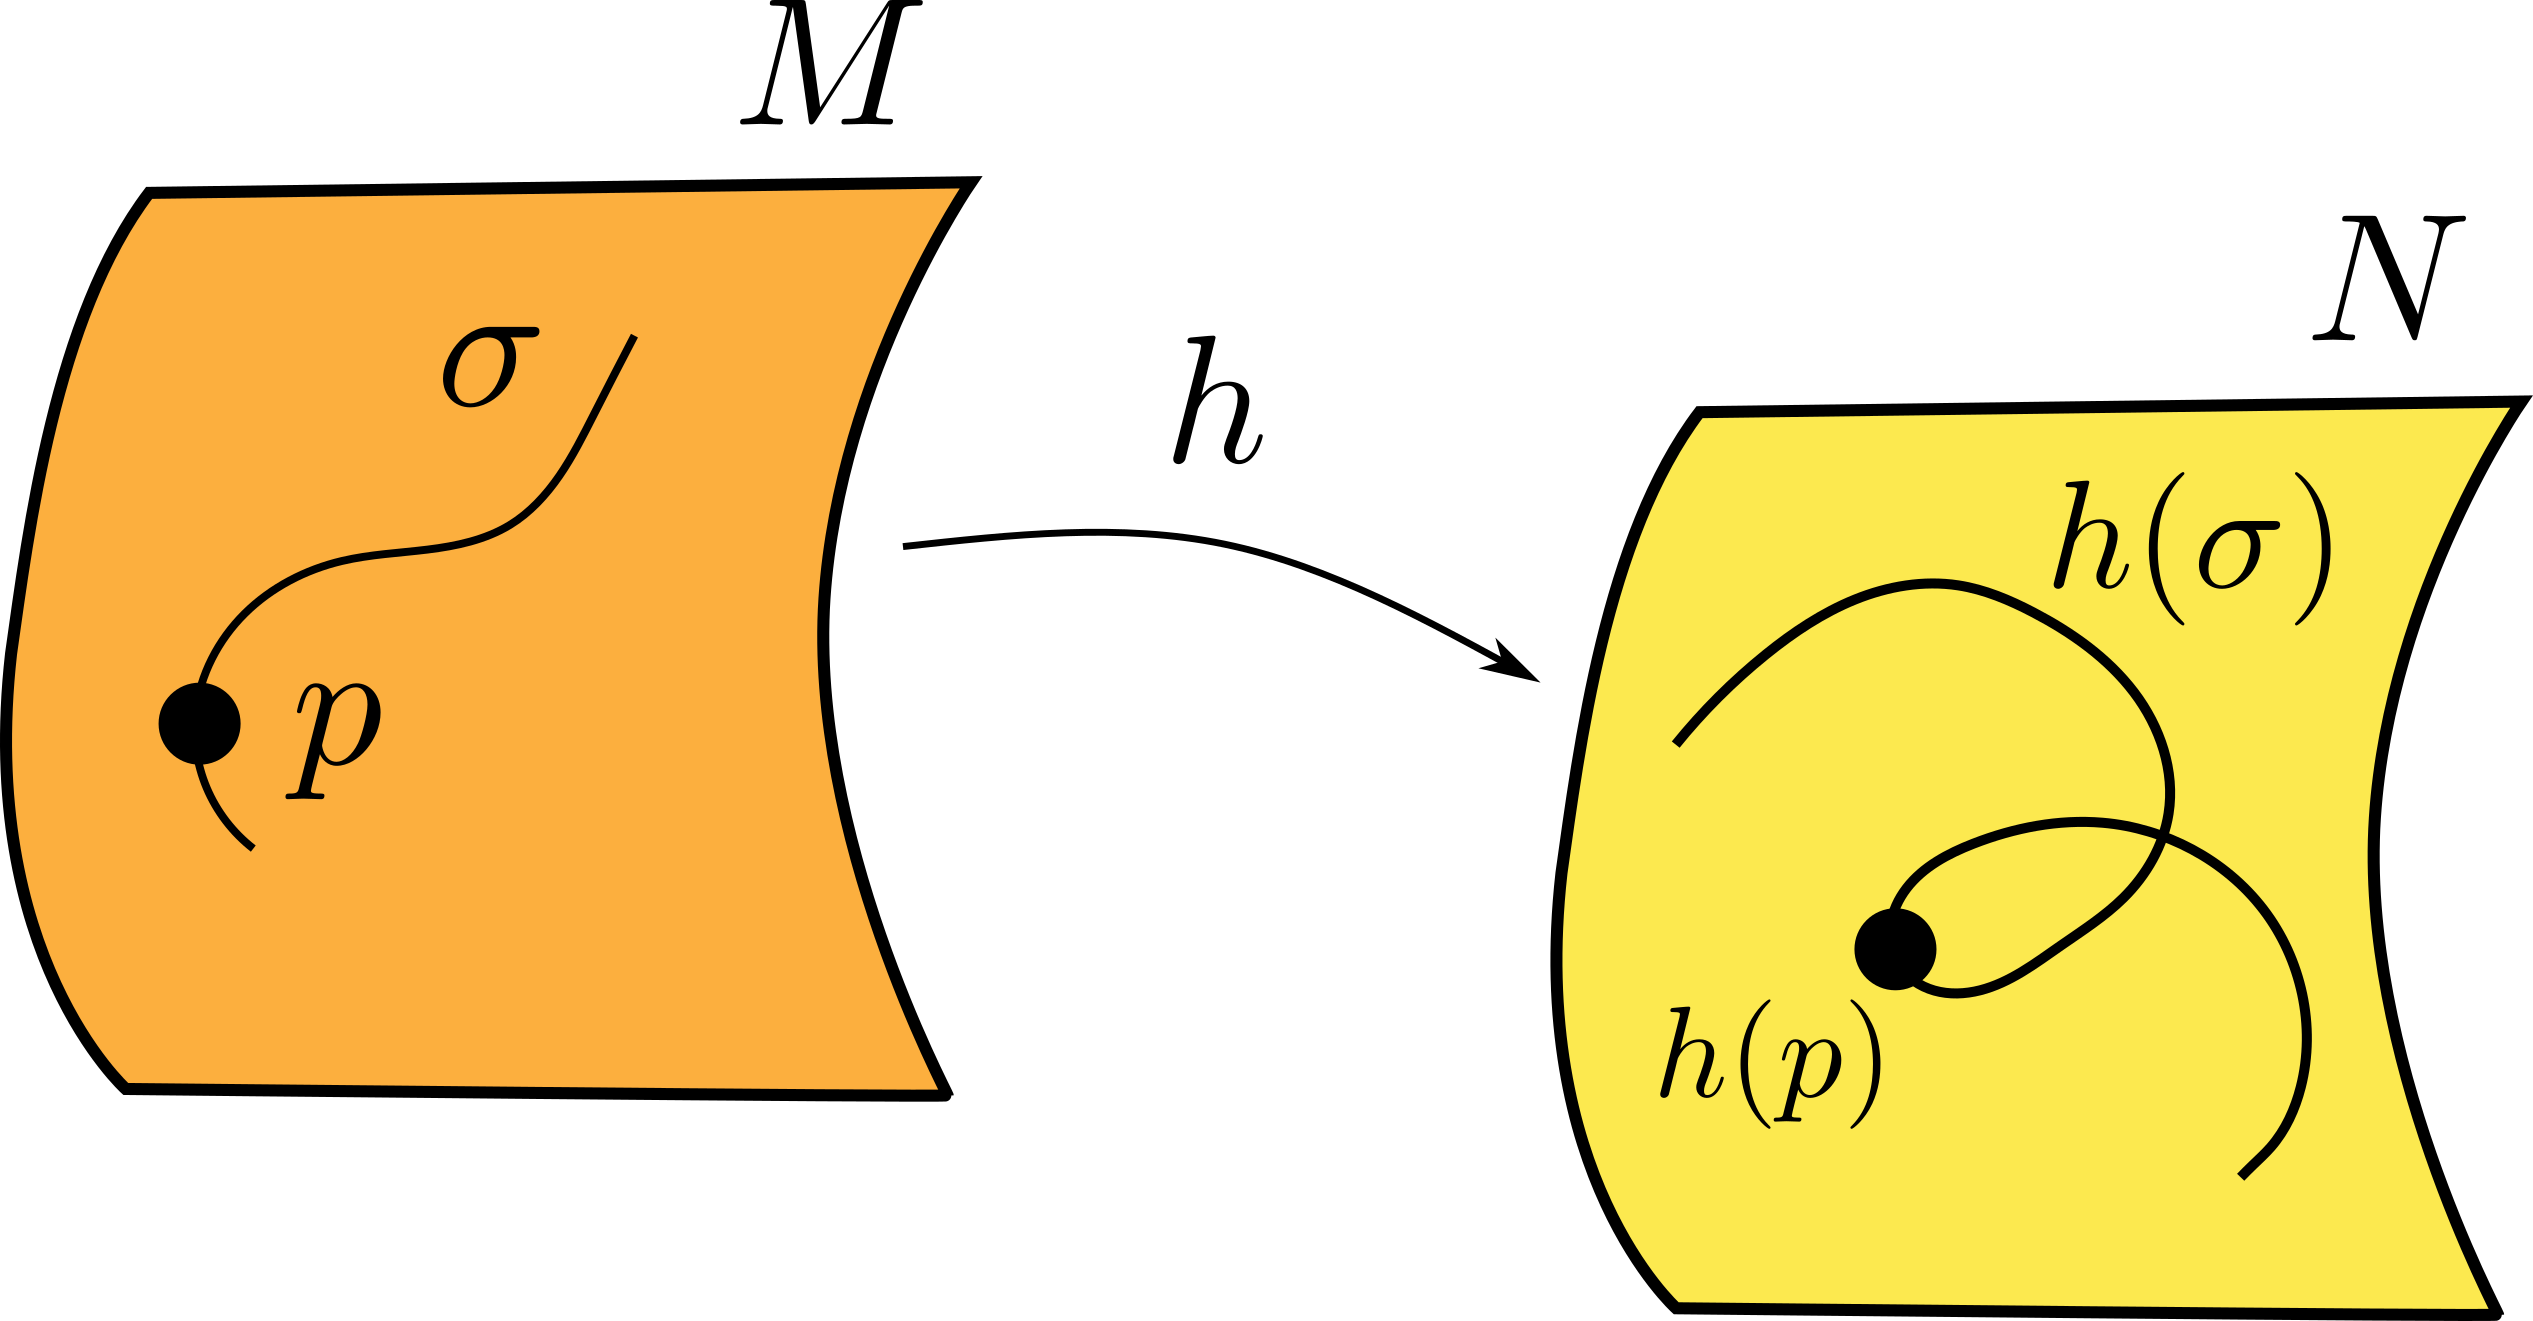
\includegraphics[width=0.4\textwidth]{fig3-1}
    \end{figure}
    Dla $v\in T_pM$, jest
    \[
        h_\star v = \frac{d}{dt}h(\sigma(t)) = h'(\sigma(t))\sigma'(t)
    ,\]
czyli $v = [\sigma] = \frac{d}{dt}\sigma(t)$,
\[
    h_\star v = \underset{\text{macierz kwadratowa}}{h'(\sigma(t))}v
.\]
\begin{przyklad}
    Niech
     \[
         S^2 = \left\{ (x,y,z)\in \mathbb{R}^3, x^2 + y^2 + z^2 = 1 \right\}
    .\]
\[
    U_1^+ = \left\{ (x,y,z)\in \mathbb{R}^3, x > 0 \right\} \cap S^2
.\]
\[
    U_1^- = \left\{ (x,y,z)\in \mathbb{R}^3, x < 0 \right\} \cap S^2
.\]
\[
    U_2^+ = \left\{ (x,y,z)\in \mathbb{R}^3, y > 0 \right\} \cap S^2
.\]
\[
    U_2^- = \left\{ (x,y,z)\in \mathbb{R}^3, y < 0 \right\} \cap S^2
.\]
\[
    U_3^+ = \left\{ (x,y,z)\in \mathbb{R}^3, z > 0 \right\} \cap S^2
.\]
\[
    U_3^- = \left\{ (x,y,z)\in \mathbb{R}^3, z < 0 \right\} \cap S^2
.\]
\begin{figure}[h]
    \centering
    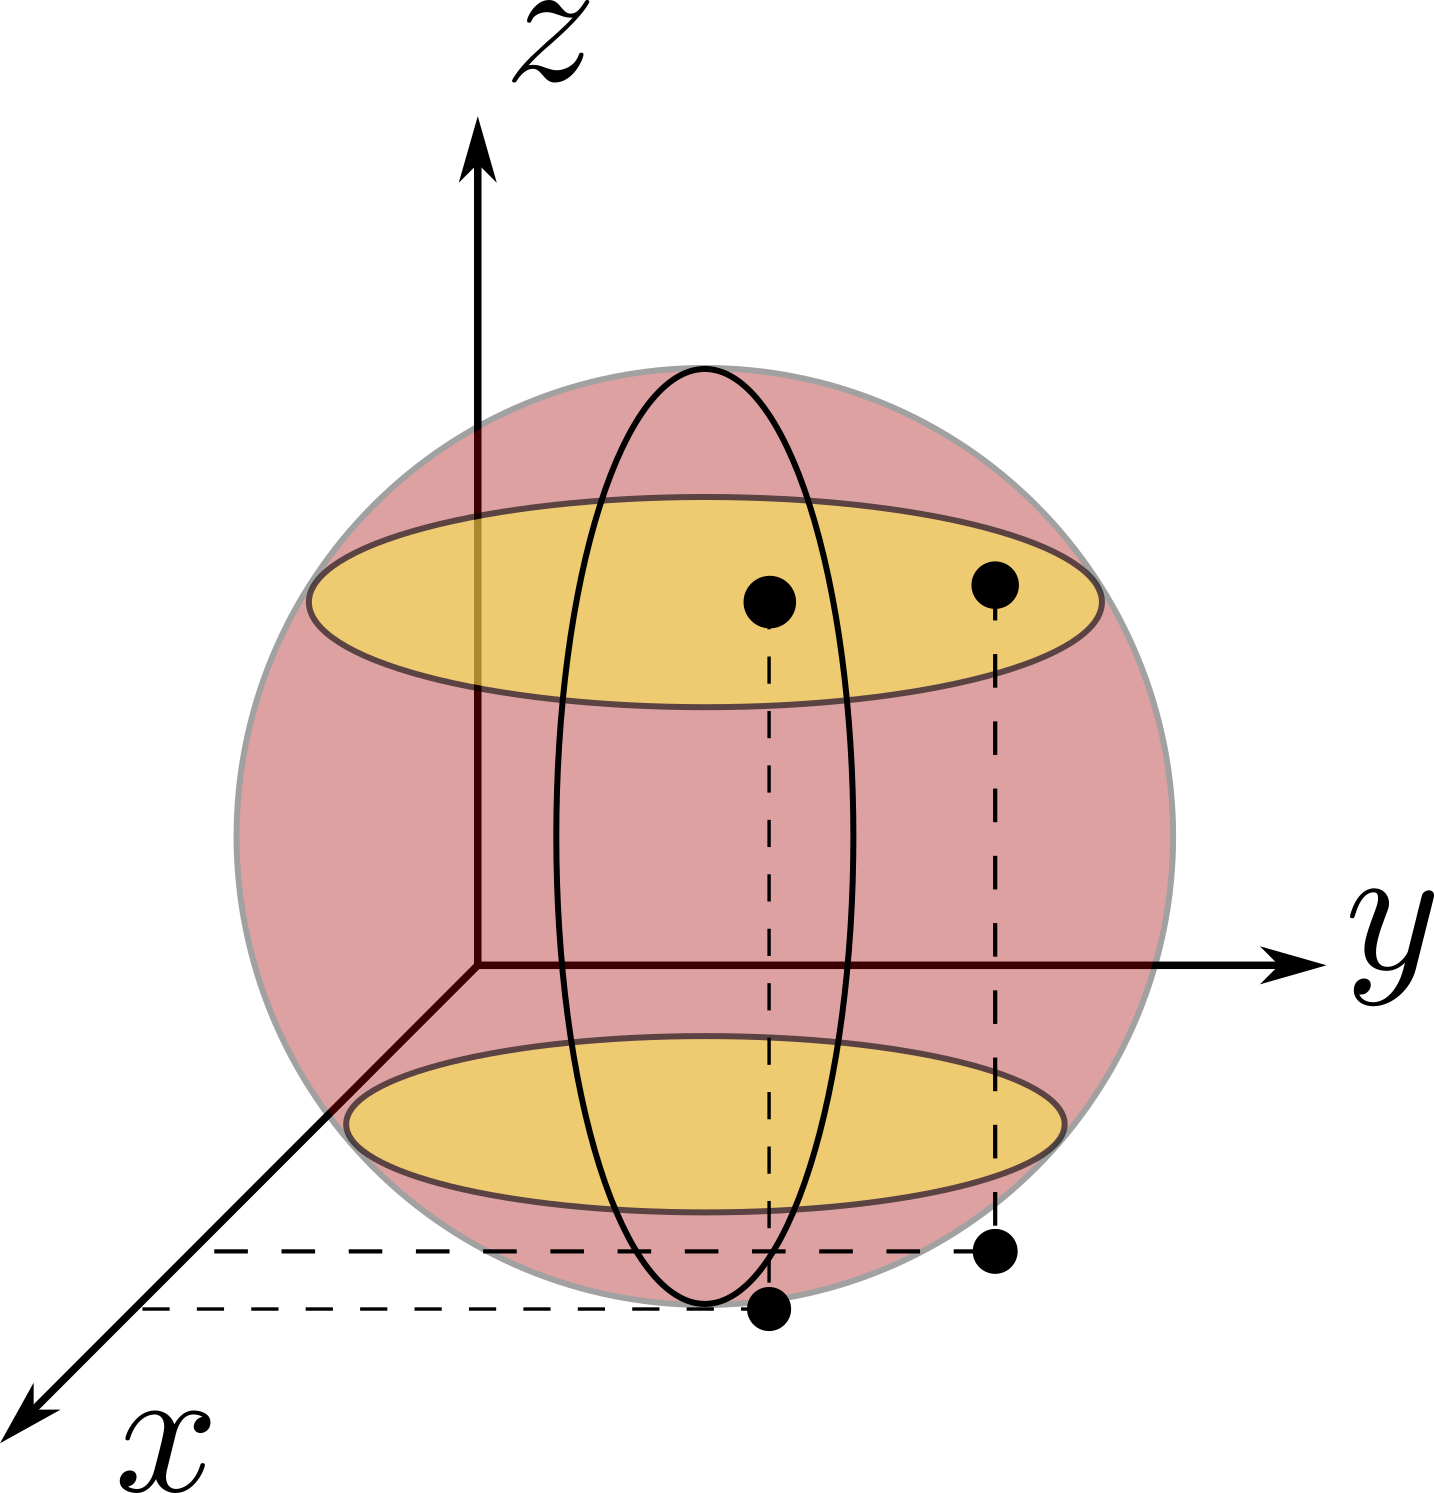
\includegraphics[width=0.3\textwidth]{fig3-2}
    \caption{Problem 3D}
    \label{fig:fig3-2}
\end{figure}
\begin{figure}[h]
    \centering
    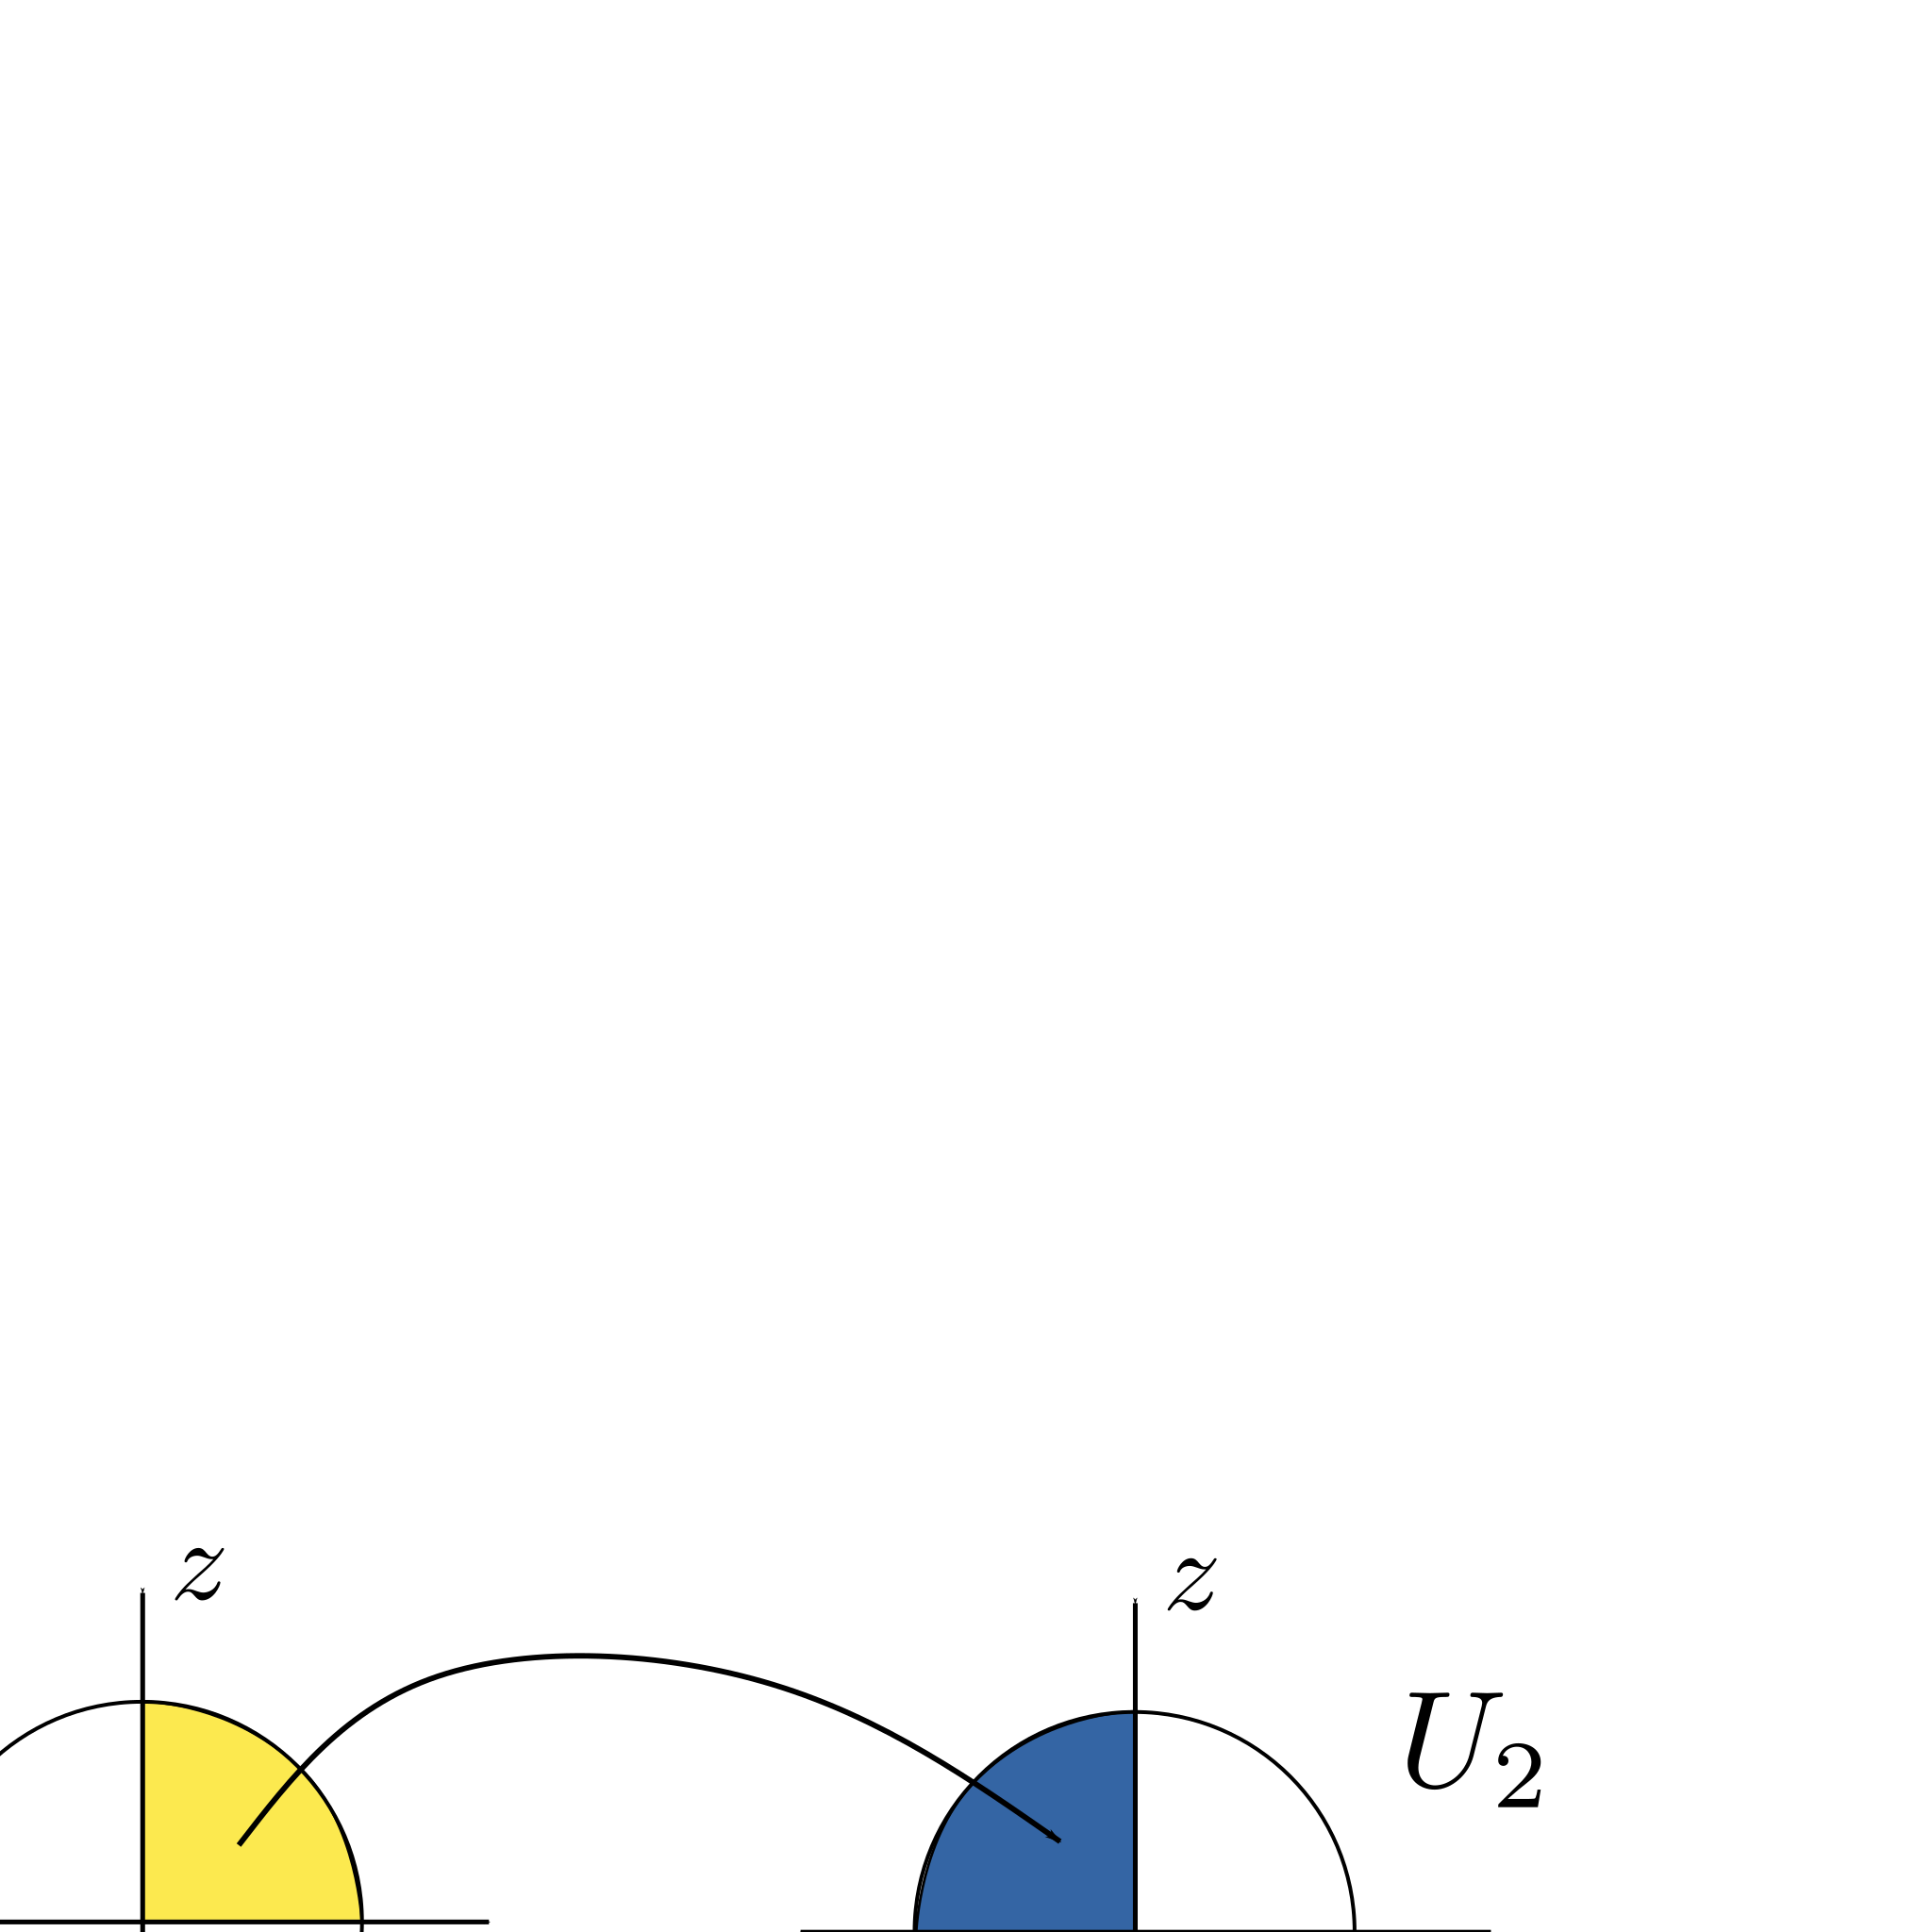
\includegraphics[width=0.4\textwidth]{fig3-3}
    \caption{mapujemy na inny}
    \label{fig:fig3-3}
\end{figure}
    Te mapy przerzucają (rys \ref{fig:fig3-2}) na np. (rys \ref{fig:fig3-3}).\\
\begin{align*}
    y &= \sqrt{1-x^2-z^2}\\
    z &= z &(z,x) \to h(z,x) = \begin{bmatrix} z\\ \sqrt{1 - x^2 - z^2} \end{bmatrix}\\
    &(x > 0, z > 0)
.\end{align*}
\[
    h' = \begin{bmatrix} \frac{\partial }{\partial z} \left( \sqrt{1-x^2-z^2}  \right) & \frac{\partial }{\partial x} \left( \sqrt{1-x^2-z^2}  \right) \\ \frac{\partial }{\partial z} \left( z \right) & \frac{\partial }{\partial x} (z) \end{bmatrix} = \begin{bmatrix} \frac{-2z}{2\sqrt{1-x^2-z^2} } & \frac{-2x}{2\sqrt{1-x^2-z^2} }\\ 1&0 \end{bmatrix}
.\]
\[
    \det h' = \frac{x}{\sqrt{1-x^2-z^2} } > 0,\quad \begin{matrix}x>0\\z>0\end{matrix}
.\]
\end{przyklad}
\begin{przyklad}
    Wstęga Moebiusa zbudowana z walca o wysokości $2L$ i promieniu $R$.
    (rys \ref{fig:fig3-4})\\
    \begin{align*}
        x(\theta, t) &= \left( R - t\sin\left(\frac{\theta}{2}\right)\right)\sin\theta\\
        y(\theta, t) &= \left( R - t\sin\left(\frac{\theta}{2}\right)\right)\cos\theta\\
        z(\theta, t) &= \left( t\cos\frac{\theta}{2}\right)
    .\end{align*}
    To jeszcze nie jest bijekcja - potrzebna druga mapa.\\
    Mamy $\theta'$ i $t'$.
    \begin{align*}
        x'(\theta',t') &= \left(R - t'\sin\left(\frac{\frac{\pi}{2} + \theta'}{2}\right)\right)\cos\theta'\\
        y'(\theta',t') &= -\left(R - t'\sin\left(\frac{\frac{\pi}{2} + \theta'}{2}\right)\right)\sin\theta'\\
        z'(\theta',t') &= t' \cos\left(\frac{\frac{\pi}{2} + \theta'}{2}\right)
    .\end{align*}
    Obszary wspólne: (rys \ref{fig:fig3-5})
    \begin{align*}
        W_1 &= \left\{ 0<\theta<\frac{\pi}{2} \right\} = \left\{ \frac{3}{2}\pi < \theta' < 2\pi \right\}\\
        W_2 &= \left\{ \frac{\pi}{2} < \theta < 2\pi \right\} = \left\{ 0 < \theta' < \frac{3}{2}\pi \right\}
    .\end{align*}
    Dla $W_1$
    \[
        \begin{cases}
            \theta' &= \theta + \frac{3}{2}\pi\\
            t' &= -t
        ,\end{cases}
    \]
dla $W_2$
    \[
        \begin{cases}
            \theta' &= \theta - \frac{\pi}{2}\\
            t' &= t
        .\end{cases}
    \]
    Szukamy macierzy przejścia
    \[
        \varphi_1'(\theta, t) = \begin{bmatrix} 1&0\\0&-1 \end{bmatrix},\quad \varphi_2'(\theta,t) = \begin{bmatrix} 1&0\\0&1 \end{bmatrix}
    ,\]
\[
\det \varphi_1' < 0 \quad \det \varphi_2' > 0
.\]
\end{przyklad}
\begin{figure}[h]
    \centering
    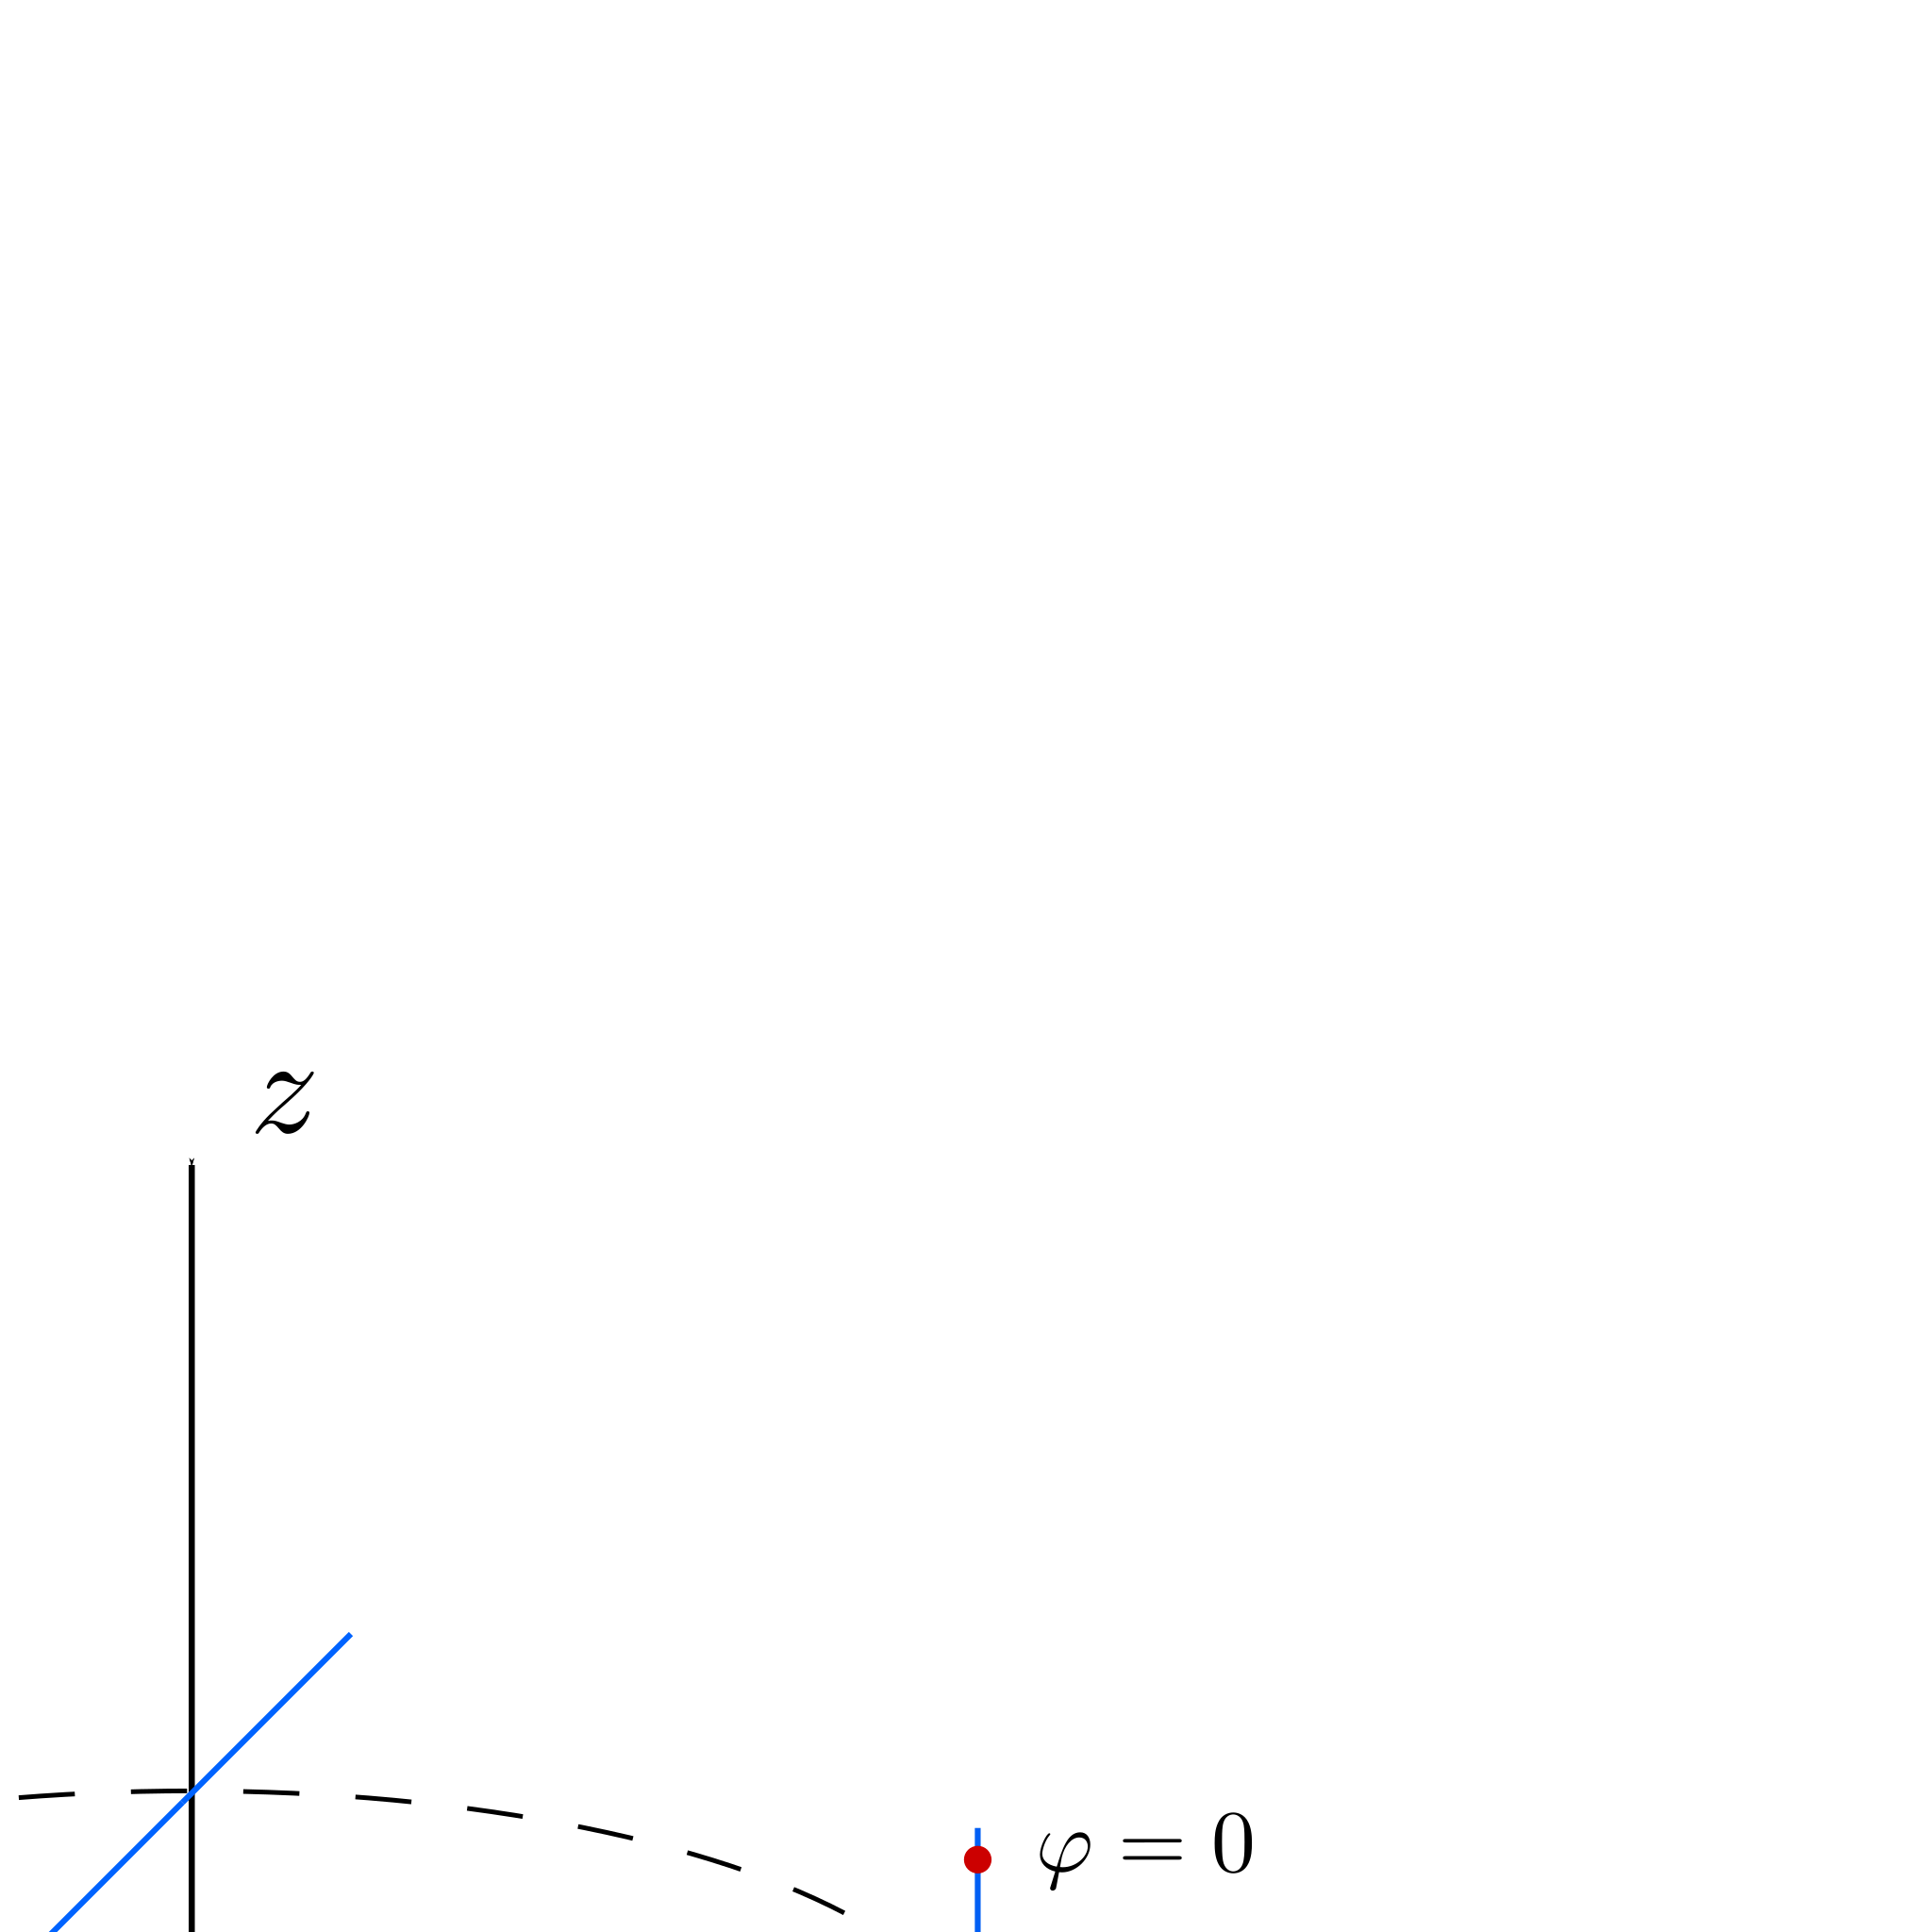
\includegraphics[width=0.45\textwidth]{fig3-4}
    \caption{Gdzie wyląduje biedronka idąc prosto po wstędze?}
    \label{fig:fig3-4}
\end{figure}
\begin{figure}[h]
    \centering
    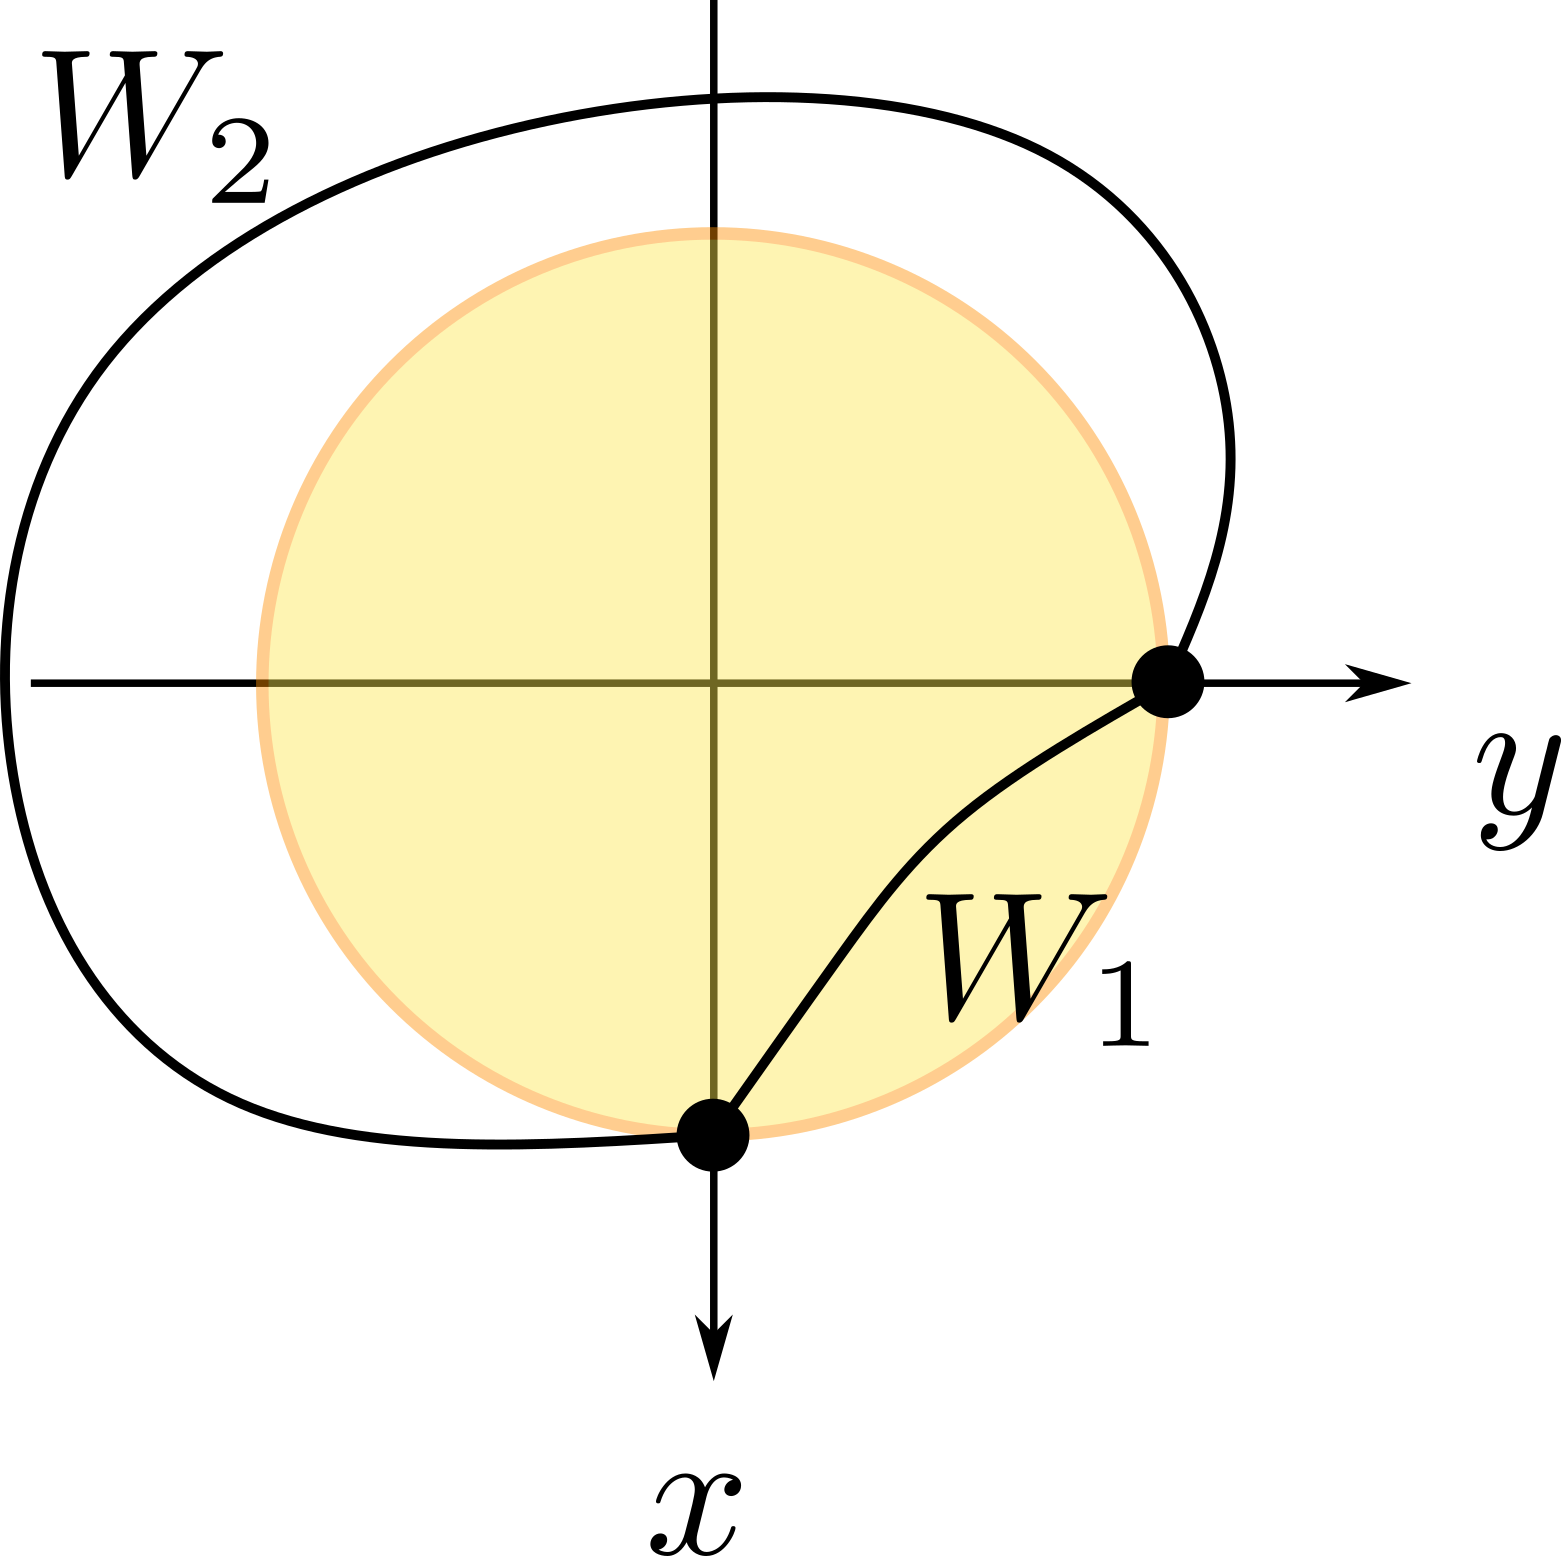
\includegraphics[width=0.35\textwidth]{fig3-5}
    \caption{Obszary wspólne}
    \label{fig:fig3-5}
\end{figure}
    \subsection{Chcemy dojść do twierdzenia Stokesa na kostce w $\mathbb{R}^n$}
    \begin{figure}[h]
        \centering
        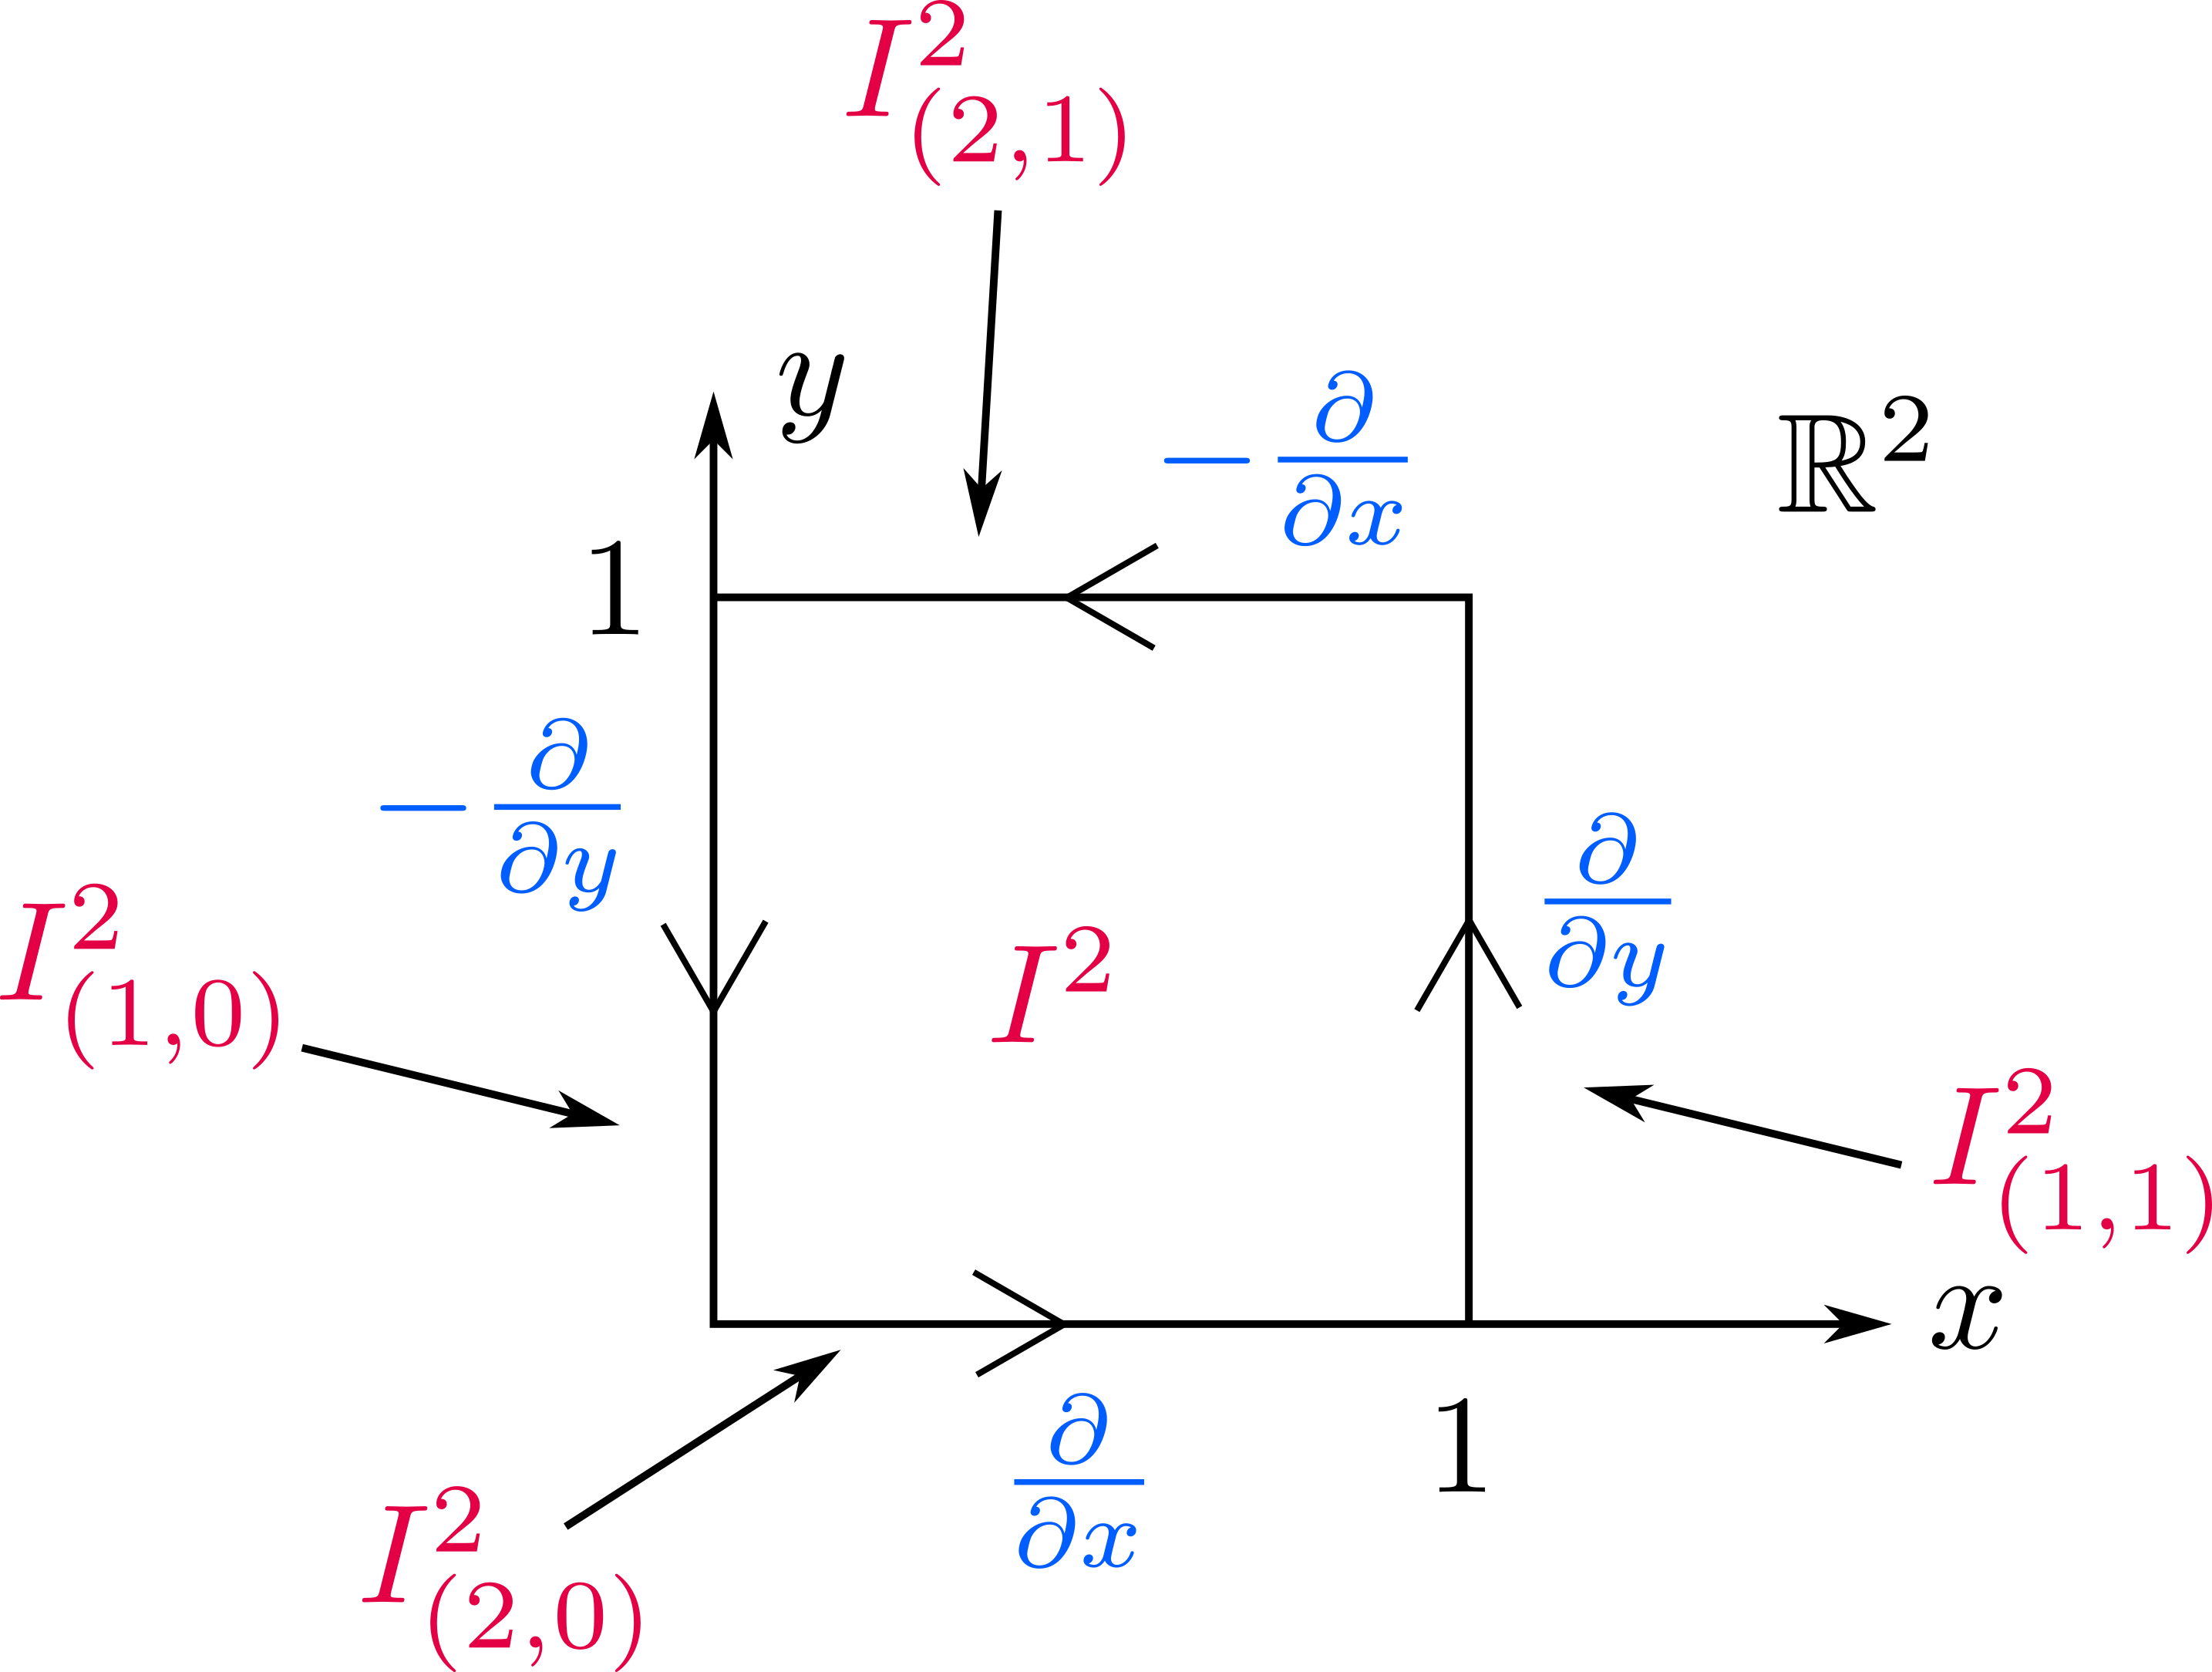
\includegraphics[width=0.4\textwidth]{fig3-6}
        \caption{Kostka w $\mathbb{R}^2$. Którędy to "na zewnątrz"?}
        \label{fig:fig3-6}
    \end{figure}
    \begin{enumerate}
        \item Niech $I^n = [0,1]\times[0,1]\times\ldots\times[0.1]\in \mathbb{R}^n$ (np. rys \ref{fig:fig3-6})\\
Wprowadźmy oznaczenia:
\[
    I^n_{(i,0)} := \left\{ \left( x^1,\ldots,x^{i-1},0,x^{i+1},\ldots,x^n \right) \in \mathbb{R}^n, 0\le x^j\le 1 \right\}
.\]
\[
    I^n_{(i,1)} := \left\{ \left( x^1,\ldots,x^{i-1},1,x^{i+1},\ldots,x^n \right) \in \mathbb{R}^n, 0\le x^j\le 1 \right\}
.\]
(odpowiednio: ścianka tylna i przednia)
\[
    \partial I^2 \overset{\text{def}}{=} I^2_{(2,0)} "=" I^2_{(1,1)} "+" - I^2_{(2,1)} "+" - I^2_{(1,0)}
,\]
(tutaj przepis na dodawanie na rysunku 6)\\
- ścianki takie zawsze będą przeciwnej orientacji.\\
Zdefiniujmy "zbiór"
\[
    \partial I^n = \sum_{i = 1}^n \sum_{\alpha = 0,1} (-1)^{\alpha + i}I^n_{i,\alpha}
,\]
który nazwiemy brzegiem zorientowanym kostki $I^n$.
    \end{enumerate}
        Niech $M$ - rozmaitość, $\dim M = n$, $I^n \in M$. Niech $\omega\in \Lambda^{n-1}(M)$. Chcemy obliczyć $\int_{\partial I^n}\omega$. Dowolna $n-1$ forma z $\Lambda^{n-1}(M)$ ma postać
        \begin{align*}
            \omega &= f_1(x^1,\ldots,x^n)dx^2\land\ldots\land dx^n +\\
            &+f_2(x^1,\ldots,x^n)dx^1\land dx^3\land\ldots\land dx^n + \ldots +\\
            &+ f_i(x^1,\ldots,x^n)dx^1\land\ldots\land dx^{i-1}\land dx^{i+1}\land \ldots\land dx^n + \ldots +\\
            &+ f_n(x^1,\ldots,x^n)dx^1\land\ldots\land dx^{n-1}
        .\end{align*}
        Ponieważ $\int_{\partial I^n}\omega$ rozbije się na $n$ składników, wystarczy, że udowodnimy Tw. Stokesa dla
        \[
            \omega = f(x^1,\ldots,x^n)dx^1\land \ldots\land dx^{i-1}\land dx^{i+1}\land \ldots \land dx^n
        .\]
    Obliczmy
    \begin{align*}
        \int_{\partial I^n}\omega &= \sum_{j=1}^n\sum_{\alpha = 0,1}(-1)^{j+\alpha} \int_{I^n(j,\alpha)} \\
        &\Bigg<f(x^1,\ldots,x^n)dx^1\land\ldots\land dx^{i-1}\land dx^{i+1}\land \ldots\land dx^n,\\
        &\frac{\partial }{\partial x^1} ,\ldots, \frac{\partial }{\partial x^{j-1}}, \frac{\partial }{\partial x^{j+1}}, \ldots, \frac{\partial }{\partial x^n}\Bigg>
        dx^1\ldots dx^{j-1}dx^{j+1}\ldots dx^n = \\
        &= \delta_{ij}\sum_{j=1}^n \sum_{\alpha = 0,1}(-1)^{j+\alpha}\int_{I^n_{j,\alpha}}f(x^1,\ldots,x^n)dx^1\ldots dx^{j-1}dx^{j+1}\ldots dx^n
    .\end{align*}
\end{document}
